\begin{mainquestion}{sourcetransform}{Source Transformations}
Use source transformations to find the voltage $V_{O}$ in the circuit below.

\begin{center}
    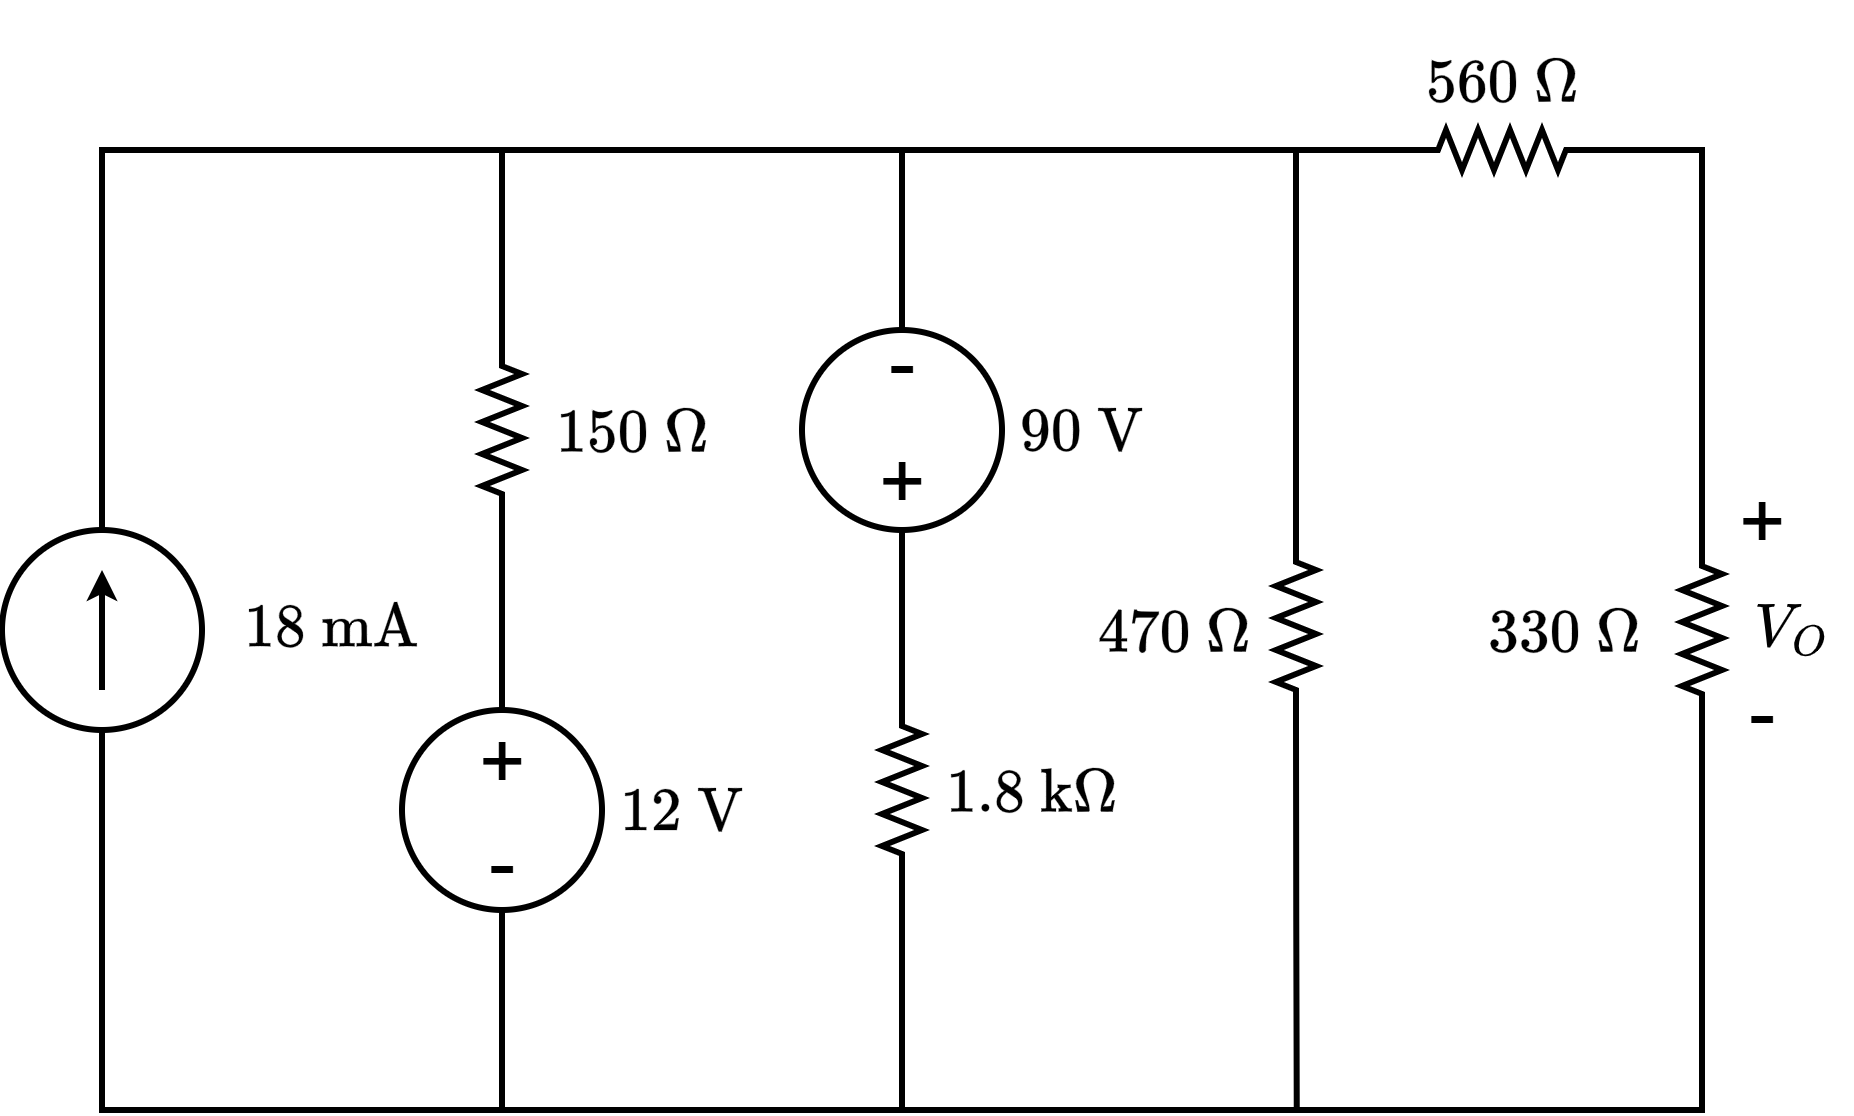
\includegraphics[width=0.8\textwidth]{questionbank/networks/source_transformations/v1/circuit.png}
\end{center}

\begin{partquestion}{findvo}{Find $V_{O}$ using source transformations.}
\begin{answer}
We first transform the 12 V source with the $150~\Omega$ series resistance into its Norton equivalent with a Norton source current of $\frac{\qty{12}{\volt}}{\qty{150}{\ohm}} = \qty{80}{\milli\ampere}$ and a Norton resistance of $150~\Omega$. Simultaneously, we can transform the 90 V source with the \qty{1.8}{\kilo\ohm} series resistance into its Norton equivalent with a Norton source current of $\frac{\qty{90}{\volt}}{\qty{1.8}{\kilo\ohm}} = \qty{50}{\milli\ampere}$ and a Norton resistance of \qty{1.8}{\kilo\ohm}. Note the polarity of the two sources are different, so the Norton current sources will be pointing in different directions! The resulting circuit looks like:

\begin{center}
    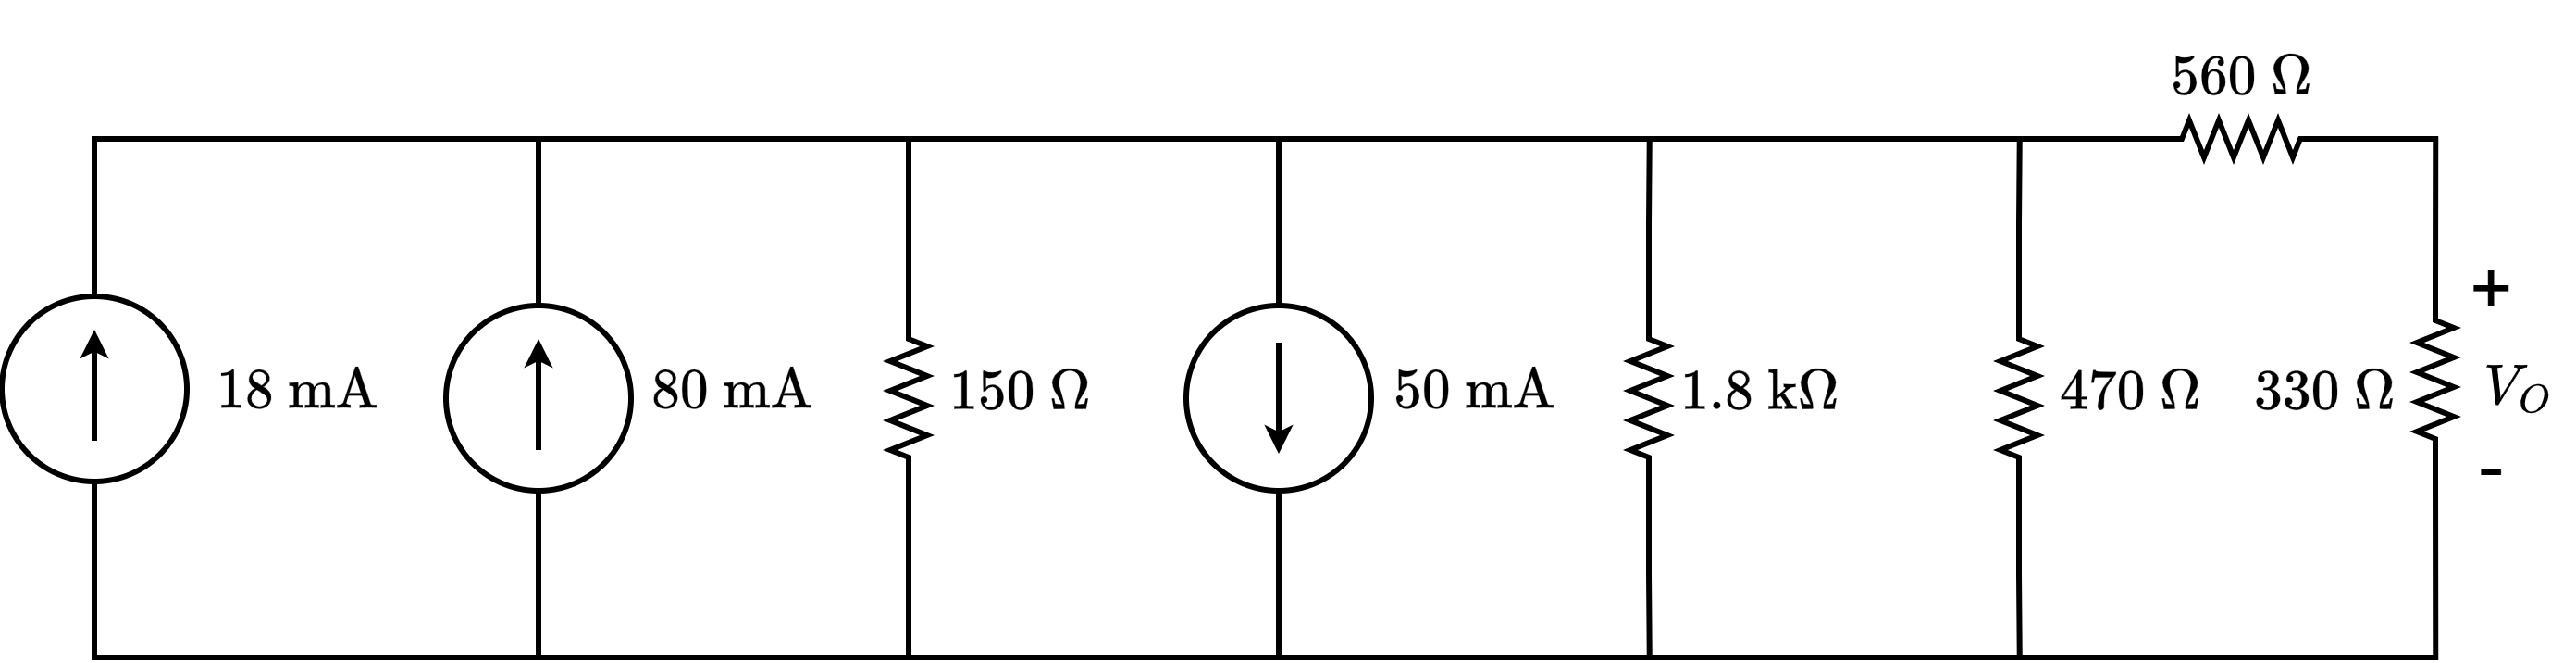
\includegraphics[width=0.8\textwidth]{questionbank/networks/source_transformations/v1/transform_1.png}
\end{center}

We can simplify the circuit considerably by combining the current sources since they are in parallel to form a \qty{48}{\milli\ampere}
source. We can also combine the three parallel resistors with a single resistor of value \qty{107}{\ohm}.
The simplified circuit looks like:

\begin{center}
    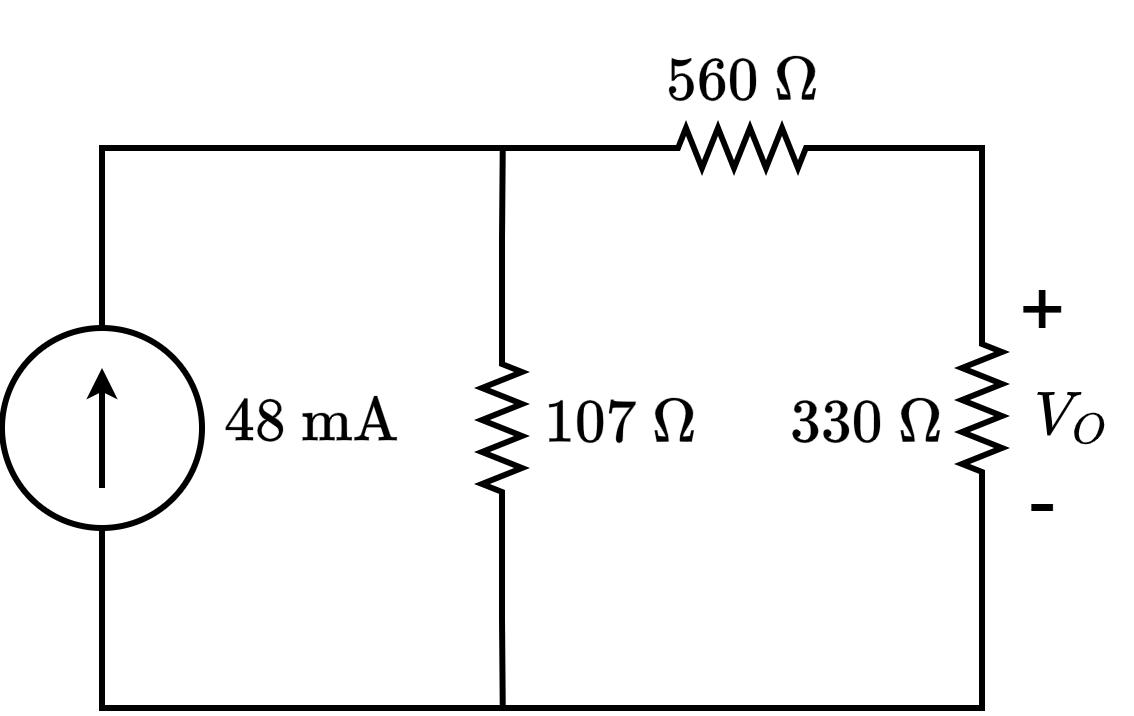
\includegraphics[width=0.5\textwidth]{questionbank/networks/source_transformations/v1/transform_2.png}
\end{center}

The next step is to apply another source transformation to a Thévenin equivalent with a Thévenin voltage source of \qty{5.13}{\volt}
with a Thévenin resistance of \qty{107}{\ohm}.
The result looks like:

\begin{center}
    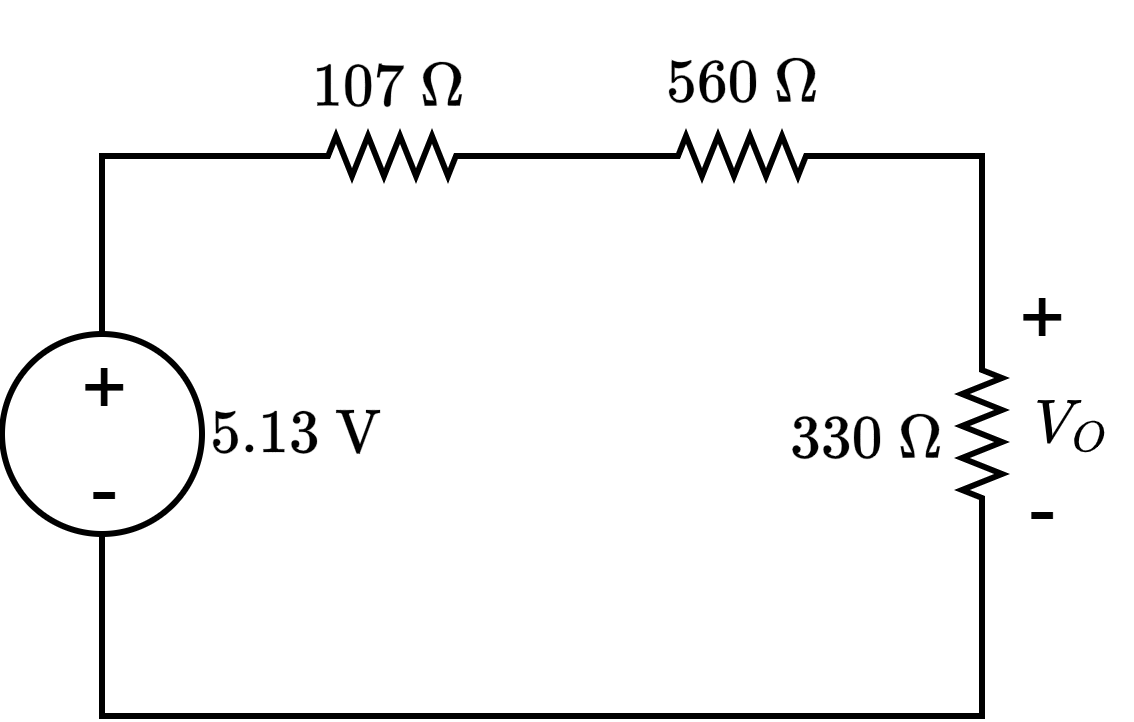
\includegraphics[width=0.5\textwidth]{questionbank/networks/source_transformations/v1/transform_3.png}
\end{center}

The result is a simple voltage divider. We can easily find the voltage across the $330~\Omega$ resistor as:
\[
V_{O}
=
5.13
\left(
\frac{330}{330+560+107}
\right)
=
\qty{1.70}{\volt}
\]
\end{answer}
\end{partquestion}

\end{mainquestion}